\section{Results} \label{sec:results}
%On the left figure \ref{fig:results1} shows a linear regression over either simulation time or time from a reference point (for patient data). On the right side of figure \ref{fig:results1}, is the superposition of an error density estimate for each data set within a category. 

\begin{sidewaysfigure} \label{fig:results1}
	\centering
	\includegraphics[trim=0cm 0cm 0cm 6cm, clip=true, scale=0.425]{figures/simulated.pdf} \\
	\includegraphics[trim=0cm 0cm 0cm 7cm, clip=true,scale=0.425]{figures/simulated_latent.pdf}\\
	\caption[Examples]{\anote{Add legend, change points, change shading, explain point colouring, explain mean and median lines.}}
\end{sidewaysfigure}

\begin{sidewaysfigure} \label{fig:res}
	\centering
	\includegraphics[trim=0cm 0cm 0cm 7cm, clip=true,scale=0.425]{figures/ancre.pdf}\\
	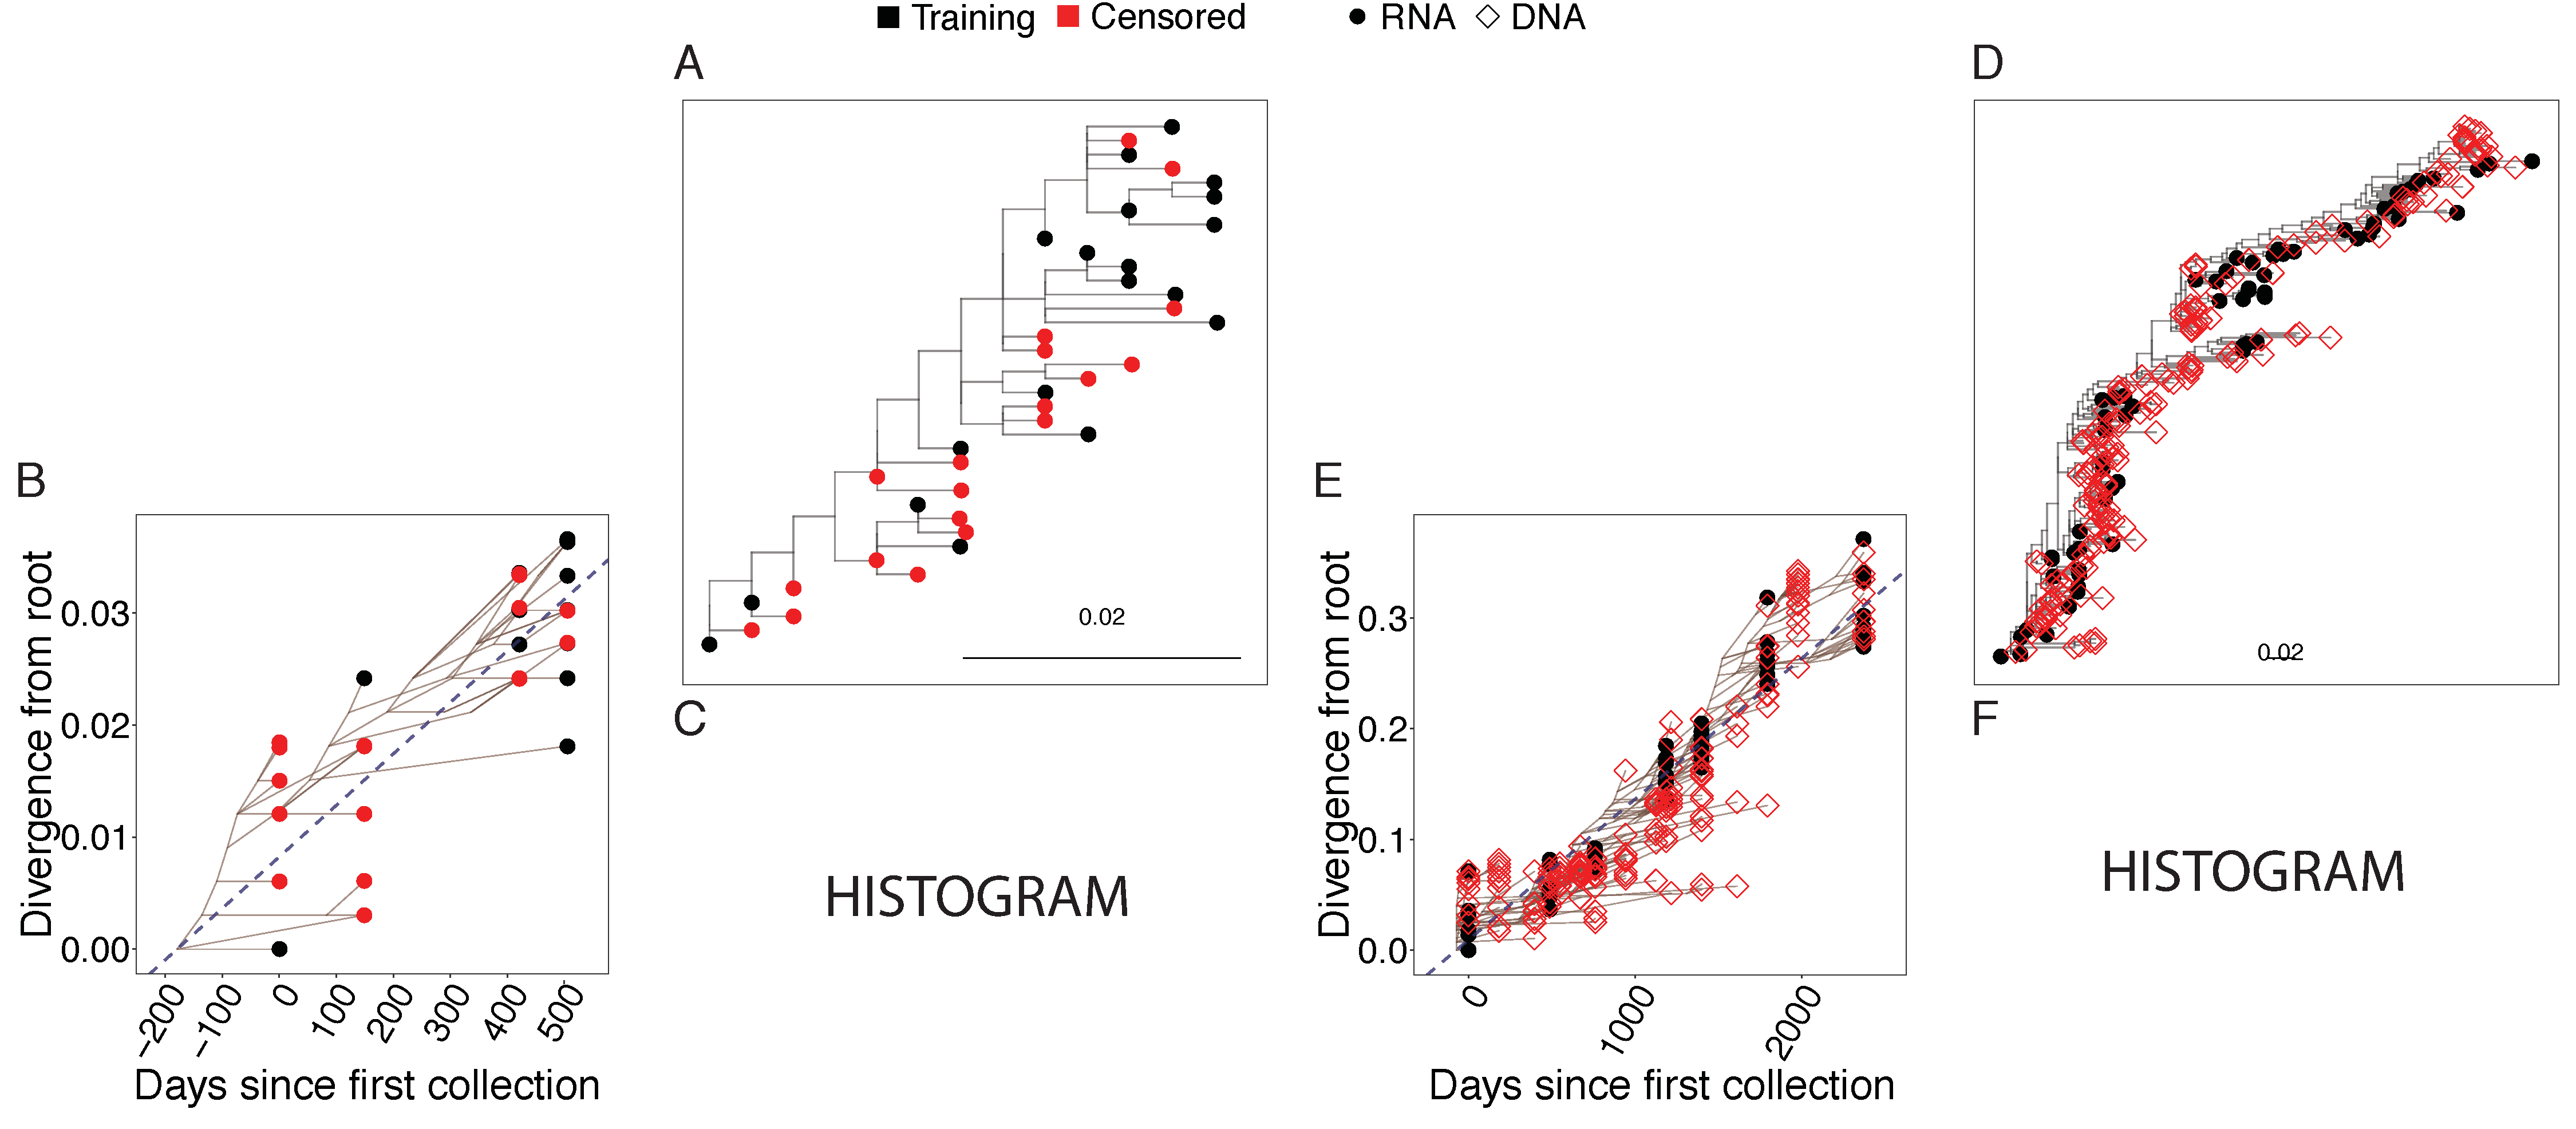
\includegraphics[trim=0cm 4cm 0cm 7cm, clip=true,scale=0.425]{figures/lanl.pdf}
	\caption[Examples]{\anote{Add legend, change points, change shading, explain point colouring, explain mean and median lines.}}
\end{sidewaysfigure}


\subsection{Simulated Data} \label{sec:sim_results}
Figure \ref{fig:results1} A shows that the clock is a reliable source of information in this case. Quantitatively, the censored data points are close to the regression line, and the difference density is heavily peaked around 0. Averaged over all simulated data sets, the average mean square error was \anote{X}, and the average median and mean difference were \anote{Y} and \anote{Z} respectively.

Figure \ref{fig:results1} B shows the regression over the calibration dates and the simulated collection dates. Note that these dates are not the actual. In this experiment, the density plot is shifted to the right, exemplifying latent behavior. Averaged over all simulated data sets, the average mean square error was \anote{X}, and the average median and mean difference were \anote{Y} and \anote{Z} respectively. However, when we utilized the known sample ages (as opposed to the collection dates) then measured the same metrics, averaged over all simulated data sets, the average mean square error was \anote{X}, and the average median and mean difference were \anote{Y} and \anote{Z} respectively.

\subsection{Plasma data-set} \label{sec:rna_only}

Figure \ref{fig:results1} C shows the regression over the calibration dates and the collection date. Averaged over all simulated data sets, the average mean square error was \anote{X}, and the average median and mean difference were \anote{Y} and \anote{Z} respectively. The superposition of the difference density plots shows similar behavior to that of \ref{sec:sim_results}, except with a wider distribution, and more variation. Since there is inherently more noise in this data, this is expected. 

\subsection{Mixed data-set} \label{sec:mixed_data}

Figure \ref{fig:results1} D shows the regression over the calibration dates and the simulated collection date. In this case, we do not know the actual date of archival.  The superposition of the difference density plots shows similar behavior to that of the latent simulated data, except \anote{need new plots for this}.  

The patients that had received treatment at some point generally failed the hypothesis testing -- there was only one patient that did not. This suggests that after a patient begins treatment, the assumption of a molecular clock over their phylogeny is too strong. 
